\documentclass[runningheads]{llncs}

% ---------------------------------------------------------------
% Include basic ECCV package
\usepackage[review,year=2026,ID=13008]{../ECCV_2026_Paper_Template/eccv}
\usepackage{../ECCV_2026_Paper_Template/eccvabbrv}
\usepackage[accsupp]{axessibility}

% ---------------------------------------------------------------
% Other packages (与主文件保持完全一致)
\usepackage{amsmath}
\usepackage{amssymb}
\usepackage{bm}
\usepackage{graphicx}
\usepackage{booktabs}
\usepackage{multirow}
\usepackage{makecell}
\usepackage{array}
\usepackage{pifont}
\usepackage{tabularx}
\usepackage{subcaption}
\usepackage[table]{xcolor}
\usepackage{url}
\usepackage[utf8]{inputenc}
\usepackage{microtype}
\usepackage{tcolorbox}
\tcbuselibrary{breakable}
\usepackage{listings}
\usepackage{todonotes}
\definecolor{skyblue}{RGB}{169, 217, 234}
%\usepackage{natbib}
\newcommand{\cmark}{{\color{green!60!black}\ding{51}}} 
\newcommand{\xmark}{{\color{red!70!black}\ding{55}}} 
\usepackage[pagebackref,breaklinks,colorlinks,citecolor=eccvblue]{hyperref}
\usepackage{colortbl}
\usepackage{orcidlink}
\newcommand{\hmark}{\textcolor{blue}{\sqrt{}\mkern-9mu{\smallsetminus}}}
\setcounter{section}{0}
\renewcommand{\thesection}{\Alph{section}}
\newcolumntype{C}{>{\centering\arraybackslash}X}

\begin{document}
% Appendices for SciIR Paper
\section{Dataset Source, License, and Compliance}
\label{sec:appendix_data_source}

To ensure full copyright compliance and transparency, we strictly limit our data sources to open-access articles licensed under \texttt{Creative Commons Attribution 4.0 International (CC BY 4.0)}. This appendix details our provenance tracking and compliance verification process.

\subsection{Data Source Scope}
Our data ingestion pipeline targets high-quality scientific figures from \textit{Nature} and \textit{Nature Communications}. We strictly filter for articles that are explicitly marked as Open Access and carry the CC BY 4.0 license.

\subsection{License Verification SOP}
We implement a rigorous two-stage Standard Operating Procedure (SOP) for license verification:
\begin{itemize}
    \item \textbf{Article-Level Verification:} We examine the article metadata to confirm the ``Open Access'' status and the presence of the specific ``CC BY 4.0'' license string.
    \item \textbf{Figure-Level Verification:} We parse the figure caption and credit line to exclude any Third-Party Material that might carry stricter copyright restrictions.
\end{itemize}

\subsection{Metadata Preservation}
For every sample in the dataset, we preserve a comprehensive metadata chain to ensure auditability:
\begin{itemize}
    \item \textbf{DOI:} Digital Object Identifier of the source article.
    \item \textbf{Article URL:} Direct link to the source.
    \item \textbf{Figure ID:} Unique identifier for the specific figure.
    \item \textbf{License Info:} Explicit License Name (CC BY 4.0) and License URL.
\end{itemize}

\subsection{Release Format and Attribution}
Our dataset release complies with CC BY 4.0 terms as follows:
\begin{itemize}
    \item \textbf{Attribution:} Each sample is accompanied by the original author attribution and a link to the source.
    \item \textbf{Indication of Changes:} We explicitly state that images have been cropped, resized, and standardized.
    \item \textbf{Derived Data:} The accompanying captions and structured annotations are released as derived datasets.
\end{itemize}

\subsection{Privacy and De-identification}
Although scientific figures typically contain low privacy risks, we enforce a default-deny policy for sensitive content:
\begin{itemize}
    \item \textbf{Faces/Identifiable Persons:} Any figure containing recognizable human faces is removed.
    \item \textbf{Patient Data:} Clinical images (X-rays, MRI, histology) or figures with potential patient IDs are excluded.
\end{itemize}


\section{Dataset Construction Pipeline}
\label{sec:appendix_construction}
\begin{figure*}[htbp] 
    \centering
    % 左侧子图：学科分布饼图
    \begin{subfigure}[b]{0.48\linewidth}
        \centering
        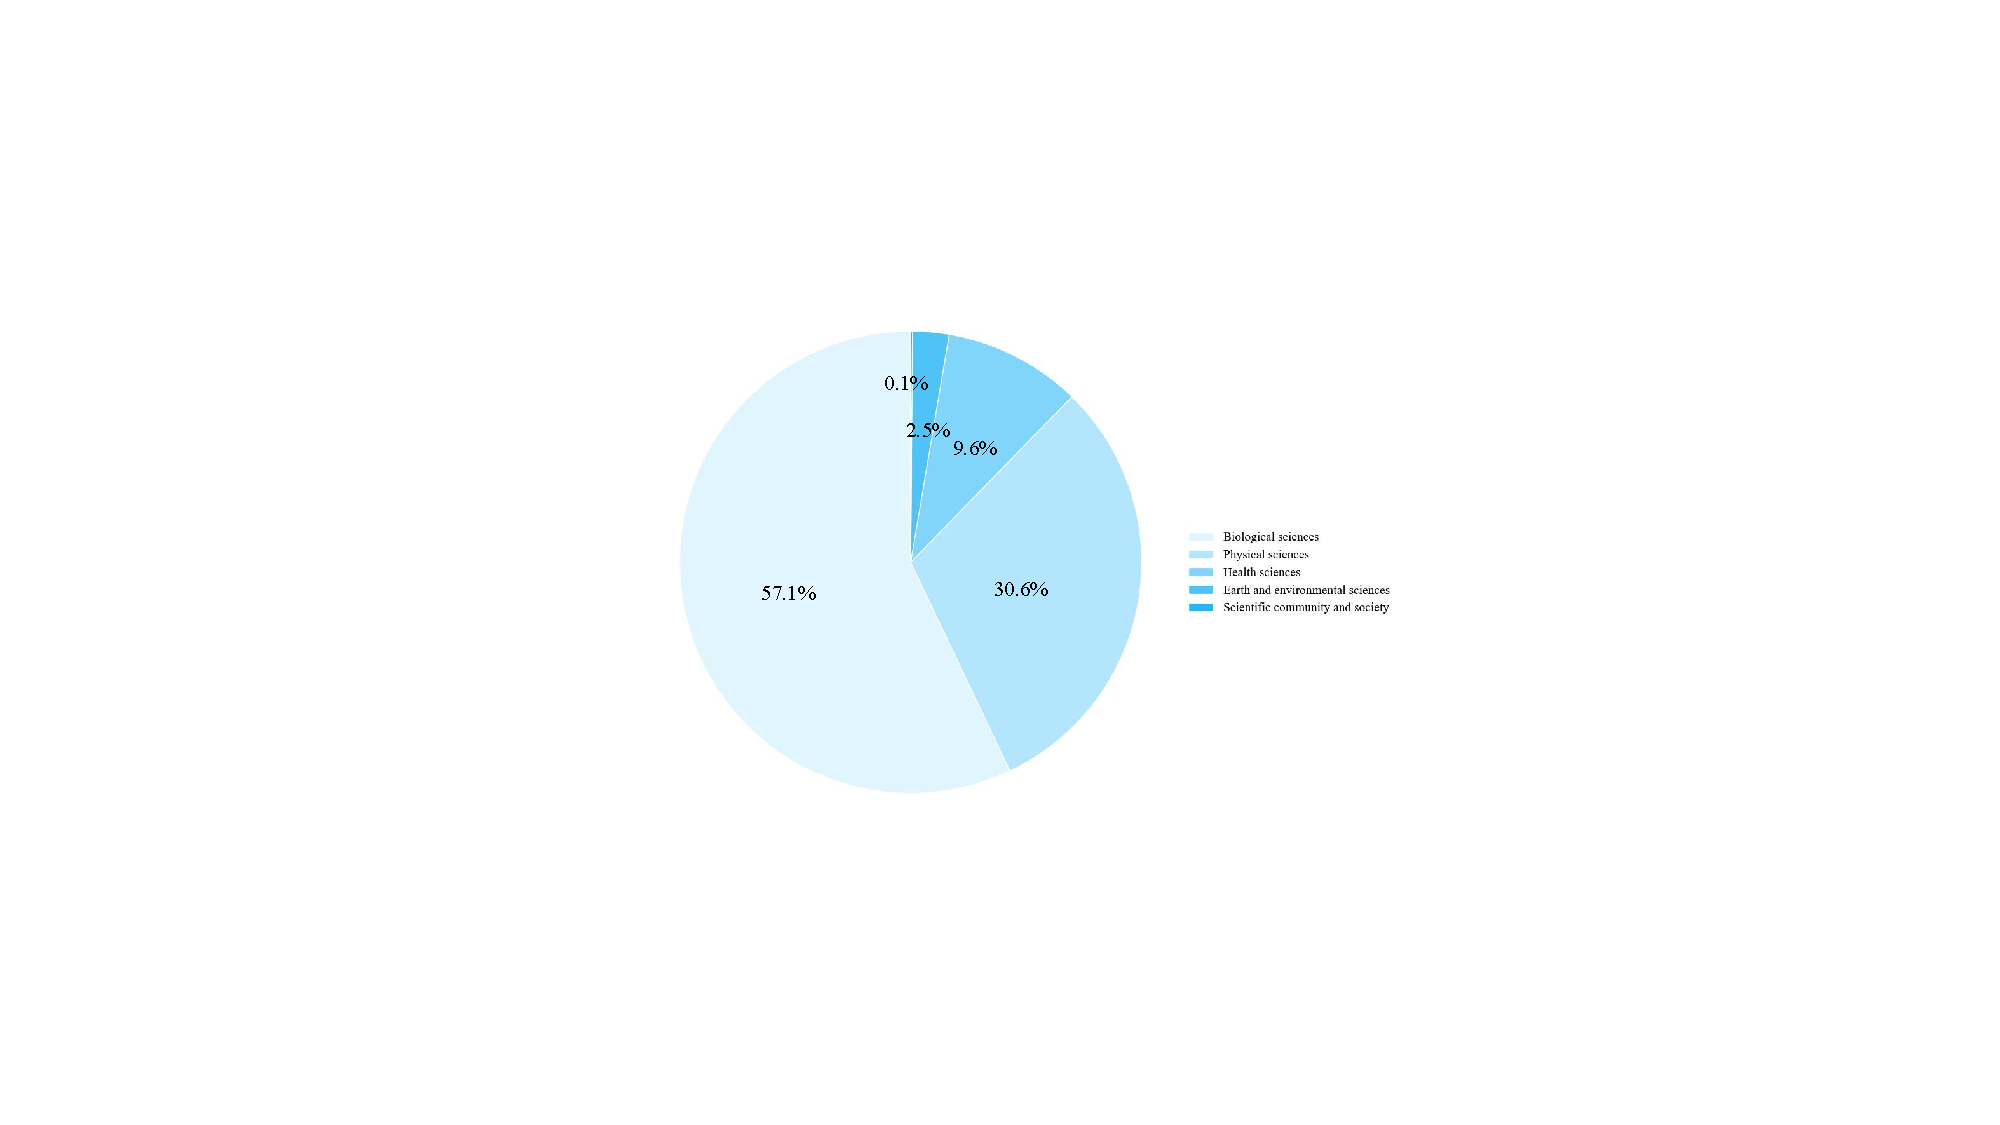
\includegraphics[width=\linewidth]{subject.pdf}
        \caption{Distribution of Figures by Discipline}
        \label{fig:discipline_pie}
    \end{subfigure}
    \hfill % 在两图之间添加弹性间距
    % 右侧子图：Term数量折线图
    \begin{subfigure}[b]{0.48\linewidth}
        \centering
        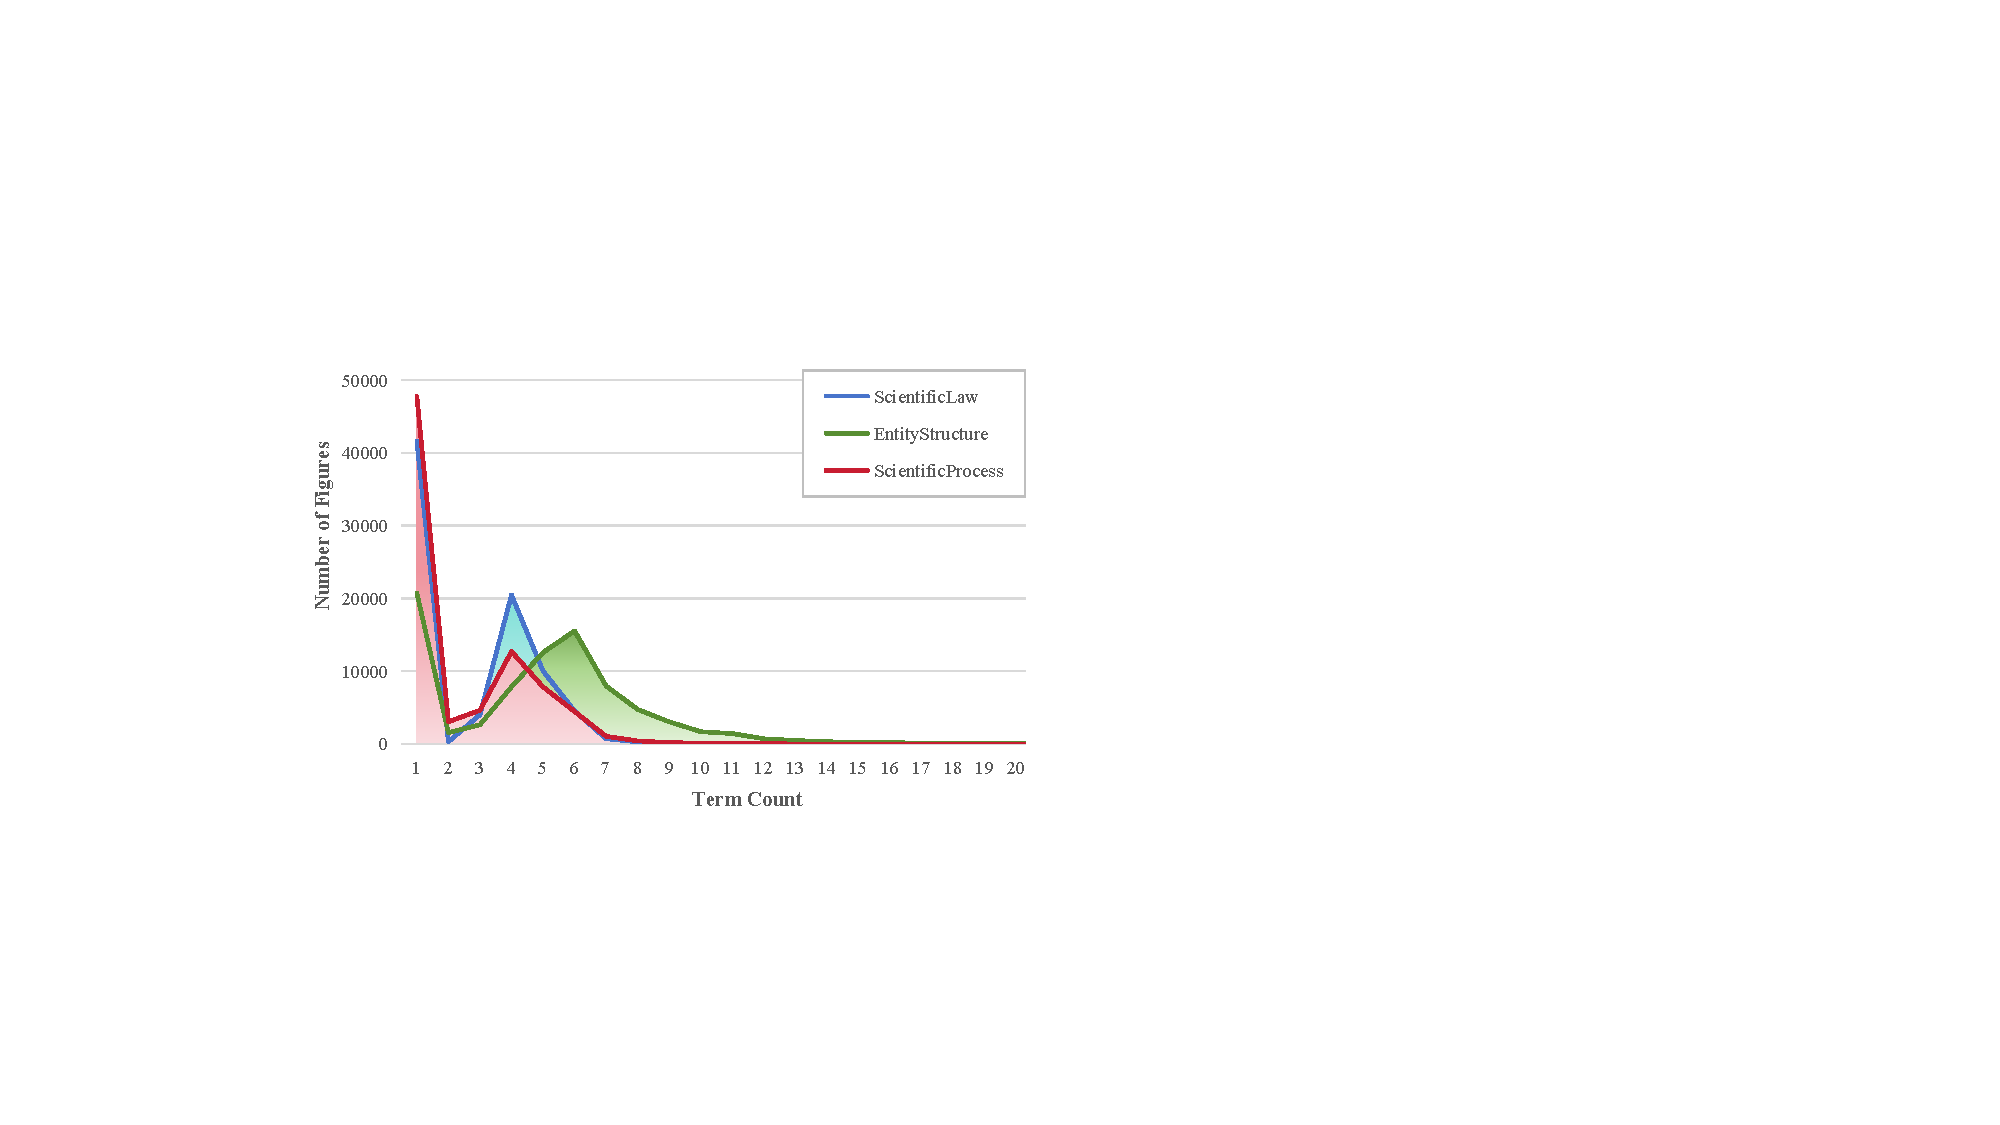
\includegraphics[width=\linewidth]{terms.pdf}
        \caption{Term Count Distribution across Tracks}
        \label{fig:term_line}
    \end{subfigure}
    
    \caption{\textbf{Dataset Statistics.} (a) The percentage of figures across different scientific disciplines. (b) The distribution of term counts for different tracks.}
    \label{fig:dataset_statistics}
\end{figure*}
\noindent
We aim for a fully reproducible image preprocessing pipeline. This section details the multi-panel splitting, standardization, and filtration mechanisms.

\begin{table}[t]
\centering
\small
% 适当增加行高，避免由于加入了横线显得上下拥挤
\renewcommand{\arraystretch}{1.15} 
\caption{Token statistics (per segment) grouped by reasoning composition.}
\label{tab:sci_rcot_token_stats_adjusted}
\setlength{\tabcolsep}{3pt} 
\resizebox{\linewidth}{!}{%
\begin{tabular}{l c c c} 
\toprule
\textbf{Reasoning Type} & \makecell{\textbf{Sci-RCoT} \\ \textbf{(mean $\pm$ std)}} & \makecell{\textbf{Prompt} \\ \textbf{(mean $\pm$ std)}} & \textbf{Ratio} \\
\midrule
% 单一类型
Entity Structure      & $212.3 \pm 69.0$ & $112.1 \pm 52.6$ & 1.89 \\
Scientific Process    & $212.7 \pm 58.2$ & $110.0 \pm 43.8$ & 1.93 \\
Scientific Law        & $267.3 \pm 73.1$ & $125.3 \pm 46.2$ & 2.13 \\
\midrule % 使用细实线进行逻辑分组
% 两两组合
Entity Structure + Scientific Process & $265.4 \pm 70.8$ & $134.8 \pm 53.1$ & 1.97 \\
Entity Structure + Scientific Law     & $250.2 \pm 71.5$ & $124.0 \pm 51.6$ & 2.02 \\
Scientific Law + Scientific Process   & $272.9 \pm 69.8$ & $136.0 \pm 51.5$ & 2.01 \\
\midrule % 使用细实线进行逻辑分组
% 三者组合
Entity Structure + Scientific Law + Scientific Process & $315.6 \pm 83.5$ & $156.5 \pm 60.1$ & 2.02 \\ 
\bottomrule
\end{tabular}% 注意这里的百分号不能漏，防止产生额外空白
}
\end{table}


\subsection{Multi-Panel Cropping}
To construct a high-quality dataset of scientific sub-figures, we implemented an automated pipeline using the fine-tuned model, which is based on the \texttt{YOLO11-Nano} architecture \cite{jocher2024ultralytics}. The pipeline consists of three stages: inference, geometric filtering, and storage.

\begin{itemize}
    \item \textbf{Model Inference Settings}
    We utilized the Ultralytics framework for inference. To accommodate varying document resolutions, input images were resized to a standard dimension of $960 \times 960$ pixels during processing. We configured the model with a confidence threshold of 0.15 to maximize recall and an Intersection over Union (IoU) threshold of 0.6 for Non-Maximum Suppression (NMS) to eliminate redundant overlapping detection boxes.
    
    \item \textbf{Post-processing}
    Raw detections specifically labeled as ``Picture'' underwent a rigorous geometric filtering process to remove noise, icons, and low-quality elements. A detected region was discarded if it met any of the following heuristic criteria:
    \begin{enumerate}
        \item \textbf{Minimum Resolution:} The width or height of the bounding box was less than 128 pixels.
        \item \textbf{Extreme Aspect Ratio:} The aspect ratio ($\text{width} / \text{height}$) fell outside the range of $[0.33, 3.0]$, ensuring that extremely narrow or flat artifacts were excluded.
        \item \textbf{Abnormal Area Occupancy:} The detection region occupied between $75\%$ and $90\%$ of the total figure area. This heuristic was specifically applied to filter out potential full-figure layout misclassifications or background elements while retaining valid single-panel figures.
    \end{enumerate}
\end{itemize}

\subsection{Image Standardization}
To ensure input consistency while preserving the original aspect ratio and visual continuity, we implemented an adaptive preprocessing workflow:

\begin{itemize}
    \item \textbf{Color Space:} All images are converted to standard RGB (sRGB), discarding transparency channels.
    \item \textbf{Resolution:} Images are unified to a fixed resolution of $1024 \times 1024$ pixels.
    \item \textbf{Adaptive Padding:} Instead of default white padding, we employ a content-aware padding strategy to minimize boundary artifacts:
    \begin{enumerate}
        \item We sample pixels from the specific edges (top/bottom or left/right) requiring extension.
        \item If a dominant color constitutes $>55\%$ of the edge pixels, it is used for padding.
        \item Otherwise, the mean RGB value of the edge pixels is calculated and applied.
    \end{enumerate}
    \item \textbf{Resampling:} We use the \texttt{Lanczos} filter for high-quality downsampling to preserve fine text and structural details during resizing.
\end{itemize}

\subsection{Dual-Stage Filtering}
We employ a cascade of automated and manual filtering to ensure high data quality.

\subsubsection{Stage 1: VLM Filtering}
We use \texttt{InternVL 3.5} to filter out low-quality or irrelevant images (e.g., photos, screenshots, pure text). The model is prompted to output a decision (KEEP/REJECT) with a reason. Items marked ``REJECT'' are discarded. Cases with low confidence are routed to manual review.

\subsubsection{Stage 2: Manual Spot-Check}
A random 10\% subset of the ``KEEP'' partition is manually reviewed to estimate the False Positive Rate (FPR). If the FPR exceeds 5\% in a batch, the filtering prompt is refined.


\subsection{Multi-Label Strategy}
We employ a soft-labeling approach that is binarized into a multi-hot encoding scheme. 
Table~\ref{tab:sci_rcot_token_stats_adjusted} summarizes the token statistics across different reasoning composition types.
\begin{itemize}
    \item \textbf{Relevance Scoring:} The VLM (Qwen3-VL) assigns a relevance score ranging from 1 to 10 for each reasoning track.
    \item \textbf{Thresholding:} A label is activated only if the assigned score satisfies $s \ge \tau$, where the threshold $\tau$ is empirically set to 7.
    \item \textbf{Data Filtering:} To ensure dataset quality, samples identified as ``low reasoning content'' (where all track scores are $<\tau$) are strictly excluded from the training set.
\end{itemize}

\section{SciIR-Bench Data Selection}
\label{sec:benchmark_construction}

To ensure the \textbf{SciIR-Bench} serves as a rigorous evaluation standard for scientific generation, we implemented a hierarchical selection pipeline to distill the raw SciIR-82k corpus into 800 high-quality test instances. The selection process is governed by three primary dimensions: Statistical Quality Control, Semiotic Intersection, and Adaptive Difficulty Stratification.

\subsection{Statistical Quality Control}
Unlike random sampling, we enforce strict data integrity constraints. We applied a distribution-based filtering mechanism using the Interquartile Range (IQR) on three key metrics derived from the automated annotation stage:

\begin{itemize}
    \item \textbf{Term Density (Information Richness):} We calculated the total number of valid scientific terms identified across the three semiotic tracks (Law, Entity, Process). Only samples with term counts falling within the interquartile range $[Q1, Q3]$ were retained. This ensures the benchmark contains samples that are neither too simplistic for evaluation nor excessively cluttered. Avoiding high-density samples prevents exceeding the spatial composition limits of current generation models, thereby mitigating uninformative failure modes.
    \item \textbf{Textual Renderability:} To evaluate text-to-image models' ability to render scientific notation, we mandated that all candidates contain valid text rendering instructions. We applied secondary IQR filters on the lengths of both \texttt{rendered\_text\_stage2} and \texttt{retained\_text\_stage3}, ensuring a balanced complexity of textual content.
\end{itemize}

\subsection{Semiotic Intersection Grouping}
To systematically evaluate the model's ability to handle multi-modal constraints, we categorized samples based on the intersection of valid reasoning paths. A sample is assigned to a group only if it possesses non-empty \texttt{terms} and \texttt{visualization} data in at least two semiotic tracks. The benchmark is bifurcated into four combinatorial groups ($N=200$ each):

\begin{itemize}
    \item \textbf{Holistic Reasoning (All\_Three):} Samples requiring simultaneous adherence to Scientific Law, Entity Structure, and Scientific Process.
    \item \textbf{Pairwise Constraints:} Three subsets covering the specific intersections of:
    \begin{enumerate}
        \item \textbf{Entity--Law:} Structural hierarchies governed by abstract physical rules.
        \item \textbf{Law--Process:} Dynamic state changes constrained by conservation laws.
        \item \textbf{Entity--Process:} Spatial transitions during experimental workflows.
    \end{enumerate}
\end{itemize}

\subsection{Adaptive Difficulty Stratification}
To disentangle instruction-following capabilities from intrinsic scientific reasoning, we implemented an automated bifurcation strategy based on semantic saturation. Within each group, we calculated the median term count ($M_{terms}$) of the filtered candidates:

\begin{itemize}
    \item \textbf{Intrinsic Reasoning (Prompt-Based):} Samples with term density below the median ($< M_{terms}$) are paired with abstract \texttt{Prompts}. This information sparsity compels the model to bridge semantic gaps using its latent domain knowledge, effectively testing its capacity for autonomous scientific reasoning.
    \item \textbf{Instruction Following (CoT-Based):} Samples with term density at or above the median ($\geq M_{terms}$) are paired with the detailed \texttt{Sci-RCoT}. Given the high complexity of these scenes, the Sci-RCoT acts as a dense visual blueprint, evaluating the model's fidelity in following fine-grained, multi-step instructions without omitting critical scientific details.
\end{itemize}

\section{Automated Evaluation Protocol}
\label{app:evaluation_protocol}

To ensure the reproducibility and rigor of our evaluation, we detail the exact implementation of the automated pipeline described in Section 4.2. The pipeline consists of two distinct stages: (1) Rule-based Checklist Generation and (2) Visual Question Answering (VQA) based Adjudication. Both stages utilize \texttt{gemini-3-pro-preview} via the Google API.

\subsection{Atomic Checklist Generation}
The checklist generation module transforms the ground-truth reasoning data into a set of binary validation questions. The generation process is governed by a strict System Instruction that enforces a two-layer validation structure.

\subsubsection{Generation Logic}
The model is instructed to function as an expert in evaluation design. The generation logic is divided into two parts:

\begin{itemize}
    \item \textbf{Layer 1: Text Check.} 
    The model iterates through all text strings explicitly required in the input prompt (e.g., labels, titles). For each string, it generates questions verifying:
    \begin{enumerate}
        \item \textbf{Spelling Correctness:} Exact string matching.
        \item \textbf{Positional Accuracy:} Only if a specific position is explicitly defined in the prompt (e.g., ``top-left''). To prevent hallucinated constraints, the model is strictly forbidden from assuming positions (e.g., ``inside'') if only vague prepositions (e.g., ``labeled'') are used.
    \end{enumerate}
    
    \item \textbf{Layer 2: Track-Customized Rules (Scientific Content).} 
    Based on the \texttt{Core Track Type} (ScientificLaw, EntityStructure, or ScientificProcess), the model decomposes complex reasoning terms into atomic visual attributes. To ensure robustness against hallucinations, we implement a \texttt{Negative Constraint Injection} strategy:
    \begin{enumerate}
        \item \textbf{Scientific Law:} Checks for ``Impossible States'' (e.g., violations of gravity, chemically impossible bonds).
        \item \textbf{Entity Structure:} Checks for structural coherence (e.g., ensuring distinct objects are not fused).
        \item \textbf{Scientific Process:} Checks for flow logic conservation (e.g., no orphaned loops or ``ghost'' steps).
    \end{enumerate}
\end{itemize}

\subsection{Automated Adjudication}
The evaluation phase employs a VLM as a ``Senior Scientific Image Reviewer.'' The model receives the generated image, the original prompt, and the checklist JSON. 

\subsubsection{Reviewer System Prompt}
To mimic human peer review, the system prompt enforces a \texttt{Chain-of-Thought (CoT)} process for every question. The model is required to execute the following steps before outputting a verdict:
\begin{enumerate}
    \item \textbf{Visual Evidence Retrieval:} Explicitly locate the specific element mentioned in the checklist question within the image.
    \item \textbf{Reasoning:} Formulate a one-sentence justification based \textit{only} on visual observation.
    \item \textbf{Verdict:} Assign a binary ``Yes'' (Pass) or ``No'' (Fail).
\end{enumerate}

\subsection{Strict Scoring Aggregation}
As detailed in the provided analysis script, our scoring metric differs from conventional VQA accuracy. We prioritize scientific exactness through a \texttt{Veto Mechanism}.

For a given image $I$ and a specific category $C$ (e.g., Scientific Law), the image is considered valid ($V_{I,C} = 1$) if and only if it passes all atomic questions $q$ belonging to that category:
\begin{equation}
    V_{I,C} = \prod_{q \in Q_{I,C}} \mathbb{I}(\text{Answer}(q) = \text{``Yes''})
\end{equation}
where $\mathbb{I}$ is the indicator function. If a single check fails (e.g., one misspelled label or one incorrect arrow direction), the entire sample is marked as a failure for that category. The final Pass Rate reported in our benchmarks is the percentage of valid samples across the dataset.
\section{Experiments}
\begin{table}[t]
\centering
\caption{\textbf{Ablation Study}.}
\label{tab:ablation_study}

\small
\setlength{\tabcolsep}{5pt}
\renewcommand{\arraystretch}{1.15}

\begin{tabular}{lccccc}
\toprule
\textbf{Variant} & \textbf{SL} & \textbf{ES} & \textbf{SP} & \textbf{Text} & \textbf{Final} \\
\midrule
Qwen-Image-2512 & 40 & 50 & 37 & 15 & 35 \\
w/o Sci-RCoT    & 41 & 54 & 39 & 15 & 38 \\
w/o Planner     & 42 & 56 & 49 & 14 & 41 \\
w/o Taxonomy    & 41 & 54 & 45 & 15 & 39 \\
\textbf{Full}
& \cellcolor{skyblue!35}\textbf{43}
& \cellcolor{skyblue!35}\textbf{59}
& \cellcolor{skyblue!35}\textbf{53}
& \cellcolor{skyblue!35}\textbf{15}
& \cellcolor{skyblue!35}\textbf{43}
\\
\bottomrule
\end{tabular}
\end{table}

\begin{table}[t]
\centering
\caption{\textbf{Effect of Judge}.}
\label{tab:judge_sensitivity}

\small
\setlength{\tabcolsep}{4pt}
\renewcommand{\arraystretch}{1.15}

\begin{tabular}{lcccc}
\toprule
\textbf{Model}
&
\textbf{Gemini}
&
\textbf{GPT-5.5}
&
\textbf{Claude-4.6}
&
\textbf{Qwen3.5}
\\
\midrule
Nano-Banana-Pro
& \cellcolor{skyblue!35}\textbf{95}
& \underline{95}
& 97
& 99 \\

GPT-Image-1
& \cellcolor{skyblue!35}\textbf{62}
& 67
& \underline{65}
& 75 \\

Qwen-Image-SciIR
& \cellcolor{skyblue!35}\textbf{43}
& \underline{44}
& 46
& 54 \\

Qwen-Image-2512
& \underline{35}
& \cellcolor{skyblue!35}\textbf{34}
& 38
& 45 \\

Flux-Dev
& \underline{9}
& \cellcolor{skyblue!35}\textbf{8}
& 13
& 19 \\

BAGEL-7B-MoT
& \cellcolor{skyblue!35}\textbf{2}
& \underline{2}
& 3
& 14 \\
\bottomrule
\end{tabular}
\end{table}

\begin{table}[t]
\centering
\caption{\textbf{Effect of Criteria}.}
\label{tab:aggregation_sensitivity}

\small
\setlength{\tabcolsep}{7pt}
\renewcommand{\arraystretch}{1.15}

\begin{tabular}{lccc}
\toprule
\textbf{Model}
&
\textbf{Strict}
&
\textbf{80\% Thr.}
&
\textbf{Avg. Pass}
\\
\midrule
Nano-Banana-Pro
& \cellcolor{skyblue!35}\textbf{95}
& \underline{97}
& 98 \\

GPT-Image-1
& \cellcolor{skyblue!35}\textbf{62}
& \underline{69}
& 80 \\

Qwen-Image-SciIR
& \cellcolor{skyblue!35}\textbf{43}
& \underline{50}
& 68 \\

Qwen-Image-2512
& \cellcolor{skyblue!35}\textbf{35}
& \underline{46}
& 65 \\

Flux-Dev
& \cellcolor{skyblue!35}\textbf{9}
& \underline{11}
& 28 \\

BAGEL-7B-MoT
& \cellcolor{skyblue!35}\textbf{2}
& \underline{3}
& 11 \\
\bottomrule
\end{tabular}
\end{table}


\begin{table}[t]
\centering
\caption{\textbf{Effect of Checklist}.}
\label{tab:wording_sensitivity}

\small
\setlength{\tabcolsep}{5pt}
\renewcommand{\arraystretch}{1.15}

\begin{tabular}{lcccc}
\toprule
\textbf{Model}
&
\textbf{Original}
&
\textbf{Reordered}
&
\textbf{Violation}
&
\textbf{Concise}
\\
\midrule
Nano-Banana-Pro
& \cellcolor{skyblue!35}\textbf{95}
& \underline{96}
& 97
& 97 \\

GPT-Image-1
& \cellcolor{skyblue!35}\textbf{62}
& \underline{63}
& 71
& 67 \\

Qwen-Image-SciIR
& \cellcolor{skyblue!35}\textbf{43}
& \underline{45}
& 51
& 49 \\

Qwen-Image-2512
& \underline{35}
& \cellcolor{skyblue!35}\textbf{33}
& 44
& 41 \\

Flux-Dev
& \underline{9}
& \cellcolor{skyblue!35}\textbf{8}
& 22
& 18 \\

BAGEL-7B-MoT
& \cellcolor{skyblue!35}\textbf{2}
& \underline{5}
& 13
& 11 \\
\bottomrule
\end{tabular}
\end{table}

\begin{table}[t]
\centering
\caption{\textbf{Human Validation of Annotations}.}
\label{tab:human_audit}

\small
\setlength{\tabcolsep}{6pt}
\renewcommand{\arraystretch}{1.15}

\begin{tabular}{lcccc}
\toprule
\textbf{Task}
&
\textbf{N}
&
\textbf{Pass$\uparrow$}
&
\textbf{Minor$\downarrow$}
&
\textbf{Major$\downarrow$}
\\
\midrule
Reasoning Extraction
& 150
& 91.3
& 7.3
& 1.3 \\

Sci-RCoT
& 150
& 86.0
& 9.3
& 4.6 \\

Prompt Distillation
& 150
& 89.3
& 8.6
& 2.0 \\
\bottomrule
\end{tabular}
\end{table}

\subsection{Ablation experiments of Qwen-Image-SciIR}
To analyse the contribution of each core component of Qwen-Image-SciIR, we supplement three component-level ablation experiments: \textbf{\textit{(i)}} w/o Sci-RCoT, \textbf{\textit{(ii)}} w/o Taxonomy, and \textbf{\textit{(iii)}} w/o Planner. As reported in \cref{tab:ablation_study}, removing any component from Qwen-Image-SciIR degrades the final score.

\subsection{Stability analysis of the benchmark}
We first clarify that Qwen3-VL and InternVL3.5 are used only in the dataset construction pipeline, whereas evaluation uses only Gemini-3-Pro for checklist generation and judgment. To assess evaluation stability, we supplement stability analyses on:
\textbf{\textit{(i)}} scoring criteria,
\textbf{\textit{(ii)}} judge model,
and \textbf{\textit{(iii)}} checklist wording.
Results are shown in \cref{tab:judge_sensitivity,tab:wording_sensitivity,tab:aggregation_sensitivity}. The model rankings and main results remain stable, indicating that our evaluation results are robust to all different choices.

\subsection{Human validation}
We supplemented a human validation study on 450 random samples in SciIR-82k, which were evenly assigned to three graduate researchers with domain expertise in natural sciences. Each sample was rated along two dimensions: visual faithfulness and scientific consistency. The results are reported in \cref{tab:human_audit}.



\section{Prompts}
\label{sec:appendix_prompts}

\subsection{Taxonomy Relevance Scoring}
\begin{tcolorbox}[colback=white, colframe=blue!50!black, boxrule=1pt, arc=2mm, breakable]
\scriptsize
\begin{lstlisting}[breaklines=true, breakindent=0pt, basicstyle=\scriptsize\ttfamily, columns=fullflexible]
Role
You are a rigorous scientific image classifier. Your task is to perform multi-label, multi-dimensional relevance scoring (1-10) on the input image based on the following three dimensions.

Evaluation Dimensions and Key Points
ScientificLaw
Determine whether the image involves and presents elements related to disciplinary laws and constraints (e.g., valence states/bonds, scale relationships, visual cues of energy/momentum conservation). 
EntityStructure
Determine whether the image involves the structure and geometric relationships of scientific entities (e.g., morphology, connections, topology, and relative scale of molecules/lattices/cells/galaxies/instrument components). 
ScientificProcess
Determine whether the image presents process information (temporal evolution, causal chains, state transitions, reaction mechanisms) or has clear process clues (multi-stage labels, timelines).

Scoring Principles
Score Meaning: 1-10 represents the "relevance" of the dimension in the image, not expression intensity, correctness, or quality.
Scoring Anchors (Relevance):
1-2: Almost not involved
3-4: Sporadic clues, but very weak
5-6: Moderately relevant, some evidence
7-8: Strongly relevant, ample evidence
9-10: Dominantly relevant, core of the image

Evidence and Limitations
Answer based ONLY on visible and clear evidence in the image; do not speculate on invisible elements.
Dimension names limited to: ScientificLaw, EntityStructure, ScientificProcess.

Output Format (Strictly follow the JSON output below)
{
  "relevance": {
    "ScientificLaw": { "score": 0 },
    "EntityStructure": { "score": 0 },
    "ScientificProcess": { "score": 0 }
  }
}
\end{lstlisting}
\end{tcolorbox}

\subsection{VLM Filtering}
\begin{tcolorbox}[colback=white, colframe=blue!50!black, boxrule=1pt, arc=2mm, breakable]
\scriptsize
\begin{lstlisting}[breaklines=true, breakindent=0pt, basicstyle=\scriptsize\ttfamily, columns=fullflexible]
Role
You are an image recognition assistant. You will see some panel images segmented from scientific papers. Please judge whether the image belongs to "Scientific Illustration"."Scientific Illustration" refers to abstract and drawable scientific schematic diagrams, excluding the following categories.

Exclude the following cases:
- The image is incomplete, contains multiple independent panels, or has embedded thumbnails.
- Contains any maps, microscope images, tissue sections, biological samples, skeletal outlines, molecular structure diagrams, organ anatomical diagrams, crystal structure diagrams, etc., used to display real-world content or experimental samples.
- Rendered/simulation/3D reconstruction images generated by professional software  
  (including pseudo-color rendering effects).
- Contains only text, letters, symbols, or captions, or pure text flowcharts, pure legends, simple icons.
- Faces/Identifiable Persons: Any figure containing recognizable human faces is removed.
- Patient Data: Clinical images (X-rays, MRI, histology) or figures with potential patient IDs are excluded.

Output Requirements:
Output only one of the following two results:
- "Scientific Illustration"
- "Not Applicable"

Please judge strictly according to the definition, without extra explanation or description.
\end{lstlisting}
\end{tcolorbox}

\subsection{Reasoning Extraction}


\begin{tcolorbox}[colback=white, colframe=blue!50!black, boxrule=1pt, arc=2mm, breakable]
\scriptsize
\begin{lstlisting}[breaklines=true, breakindent=0pt, basicstyle=\scriptsize\ttfamily, columns=fullflexible]
Role
You are a scientific image reasoning annotator. Your duty is: based on the input paper text and image, extract only the scientific information explicitly supported by the image and caption, and output strict structured reasoning JSON. Do not fabricate conclusions beyond what the text and image support; do not introduce elements invisible in the image or unsupported by the caption; do not perform common sense completion. You may internally parse the input and implicitly understand the overall layout, but the final output must only contain the specified JSON fields.

Detailed Requirements:
Internally parse the input first, analyzing the overall image layout and main visual elements, prioritizing information sources: Image > Figure Title > Caption > Article Body. Note: This step is only for internal reasoning; do not list this description in the final output.

Complete the "Extracted Terms" and "Visual Description" for the corresponding information ONLY based on the selected tags in "Reasoning Ability":

ScientificLaw: Extract terms: Laws, principles, boundary conditions, applicable premises, etc. (extractable directly or implied from the graph and caption). Visualization: Manifestation of each constraint in the graph (geometric layout, labels, symbols, measurement elements, etc.).

EntityStructure: Extract terms: Scientific entity names in the image (nominalized, no verbs). Visualization: Visual characteristics of each entity (morphology, structure, color/material/texture, spatial position and scale, quantity, etc.).

ScientificProcess: Extract terms: Process names in the image (e.g., preparation process, experimental steps, time series, mechanism chain). Visualization: Visual manifestation of different stages, change conditions (e.g., arrows, timeline, loops) of this process.

Output Requirements:
Strictly follow the JSON structure below, output no extra free text.
terms: Write only terms/nouns (no sentences, punctuation, or modifiers), at the granularity confirmed by the caption and image.
visualization: For each item in terms, there must be a visual description; use concrete, restorable visual elements; do not introduce external information.
Non-empty validation: In the output JSON, "terms" and "visualization" for all selected reasoning abilities must NOT be empty lists "[]".
Unselected ability keys must be null.

Output Format:
{
  "reasoning": {
    "ScientificLaw": {
      "terms": [],
      "visualization": []
    },
    "EntityStructure": {
      "terms": [],
      "visualization": []
    },
    "ScientificProcess": {
      "terms": [],
      "visualization": []
    }
  }
}
\end{lstlisting}
\end{tcolorbox}

\subsection{Sci-RCoT Generation}
\begin{tcolorbox}[colback=white, colframe=blue!50!black, boxrule=1pt, arc=2mm, breakable]
\scriptsize
\begin{lstlisting}[breaklines=true, basicstyle=\scriptsize\ttfamily, columns=fullflexible]
Role
You are a scientific image visualization narrator. Your duty is: input reasoning, 
primarily based on the visualization items in reasoning, refer to the input image, 
and output a coherent, detailed scene description sci-RCoT.

Detailed Requirements:
1. Complete Visual Style:
   - Observe the original image, identify its specific drawing style 
     (e.g., Schematic diagram, Photorealistic render, etc.).
   - You must explicitly specify this style at the beginning of the generated instruction.

2. Complete Text Rendering:
   - Observe key text in the original image (labels, legends, axis titles).
   - You must include mandatory text rendering requirements in the instruction, 
     using phrases like "explicitly labeled as...", "including the text...", 
     "with axis labeled..." etc.

3. Integrate Scientific Logic:
   - Use the visualization items in reasoning to describe entity structure, 
     topological relationships, and dynamic processes.
   - Language must be coherent, building a complete scene, not a simple list.

Output Requirements:
Please do not output text directly, but output a JSON object containing the 
following two fields:
- "sci_RCoT": The generated complete visual description text.
- "rendered_text": A string list (List[str]), extracting all specific text 
  content you explicitly requested to render in sci_RCoT (such as label names, 
  axis titles, legend text, etc.).

Output Format (Must be strict JSON):
{
    "sci_RCoT": "Your detailed narrative...",
    "rendered_text": ["text_content_1", "text_content_2"]
}

The sci-RCoT must completely cover every point in the visualization array of 
each selected label in reasoning, without omission or altering its meaning, 
and strictly forbid adding any elements not appearing in reasoning, caption, 
or image; the language style should be concrete, coherent, and capable of 
restoring the scene from text.
\end{lstlisting}
\end{tcolorbox}

\subsection{Abstract Prompt Distillation}
\begin{tcolorbox}[colback=white, colframe=blue!50!black, boxrule=1pt, arc=2mm, breakable]
\scriptsize
\begin{lstlisting}[breaklines=true, breakindent=0pt, basicstyle=\scriptsize\ttfamily, columns=fullflexible]
Role: Scientific Image Reasoning Generation Prompt Assistant

Objective: Your goal is to generate a concise, semantically compressed abstract_prompt in JSON format. You will achieve this by synthesizing input sci-RCoT with specific Reasoning dimension terms.

Input Data:
- sci-RCoT: TA detailed image description composed of all the 'visualization' elements from 'reasoning'.
- Reasoning: Contains specific 'terms' and their corresponding 'visualization'.
- rendered_text: A list of text strings allowed to be rendered in the image.

Processing Logic:
1. Analyze: Read the sci-RCoT to understand the scientific semantics.
2. Preserve Style: Extract the visualization style requirement (typically the first sentence or phrase of sci-RCoT, e.g., "A realistic 3D render...", "A schematic diagram of...", "A cross-section view..."). This must be the opening of your abstract_prompt.
3. Map & Replace: Identify the description in sci-RCoT that corresponds to 'visualization' in Reasoning, and strictly replace it with the 'terms' provided in Reasoning.
4. Text Selection: Determine necessary text labels based on the sci-RCoT context. Include text rendering requests in abstract_prompt if they are necessary for scientific clarity or context.
5. Compress: Synthesize the result into an abstract_prompt without visual descriptions.
6. Synchronization: Extract exactly the text strings that are explicitly requested to be rendered in your generated abstract_prompt and populate the retained_text list.

Constraints & Guardrails:
- Semantic Integrity: The replacement must perfectly match the original scientific semantics.
- Style Consistency: The output must start with the original visualization style found in sci-RCoT.
- Output Format: Return only a JSON object with the following structure:
{
  "abstract_prompt": "Your concise, term-based prompt here... (e.g., 'Diagram showing [Term A] labeled 'Text1'...')",
  "retained_text": ["Text1", "Text2"]
}
\end{lstlisting}
\end{tcolorbox}

\subsection{Checklist Generation}
\begin{tcolorbox}[colback=white, colframe=blue!50!black, boxrule=1pt, arc=2mm, breakable]
\scriptsize
\begin{lstlisting}[breaklines=true, breakindent=0pt, basicstyle=\scriptsize\ttfamily, columns=fullflexible]
Role
You are an expert in evaluation design for scientific image generation benchmarks. Your task is to generate a JSON checklist for VLM scoring based on the instructions provided by the user.

Context
You need to generate checkpoints for two layers for each test sample based on the data below.

Input Data Definitions
Core Track Type: The specific track (EntityStructure, ScientificProcess, or ScientificLaw).
Input Prompt: The complete prompt containing text requirements and scientific descriptions.
Reasoning: Structured terms extracted from reference materials.

Generation Rules
Part 1: General Rules (Applies to all Prompts)
Layer 1 - Text Check (Text Rendering):
Input Processing:
ITERATE through all text explicitly required for rendering in the Input Prompt (look for quotes, "Label...", "Text...").
Execution:
FOR EACH text item found:
GENERATE a specific question checking:
"Spelling Correctness"
"Positional Accuracy" (IF AND ONLY IF the position is explicitly specified in the Prompt).
Negative Constraints (CRITICAL):
SCOPE: Questions must ONLY evaluate the text string itself (Spelling, Existence, Position).
NO VISUALS: Do NOT verify visual attributes of the object the text is on (e.g., ignore color, shape, arrow direction).
NO HALLUCINATION: Strictly based on the position described in the original text; speculation is prohibited. 
Category: "Text"

Part 2: Track-Customized Rules (Core Scientific Content)
Mapping and Filtering Logic:
Select Term Source: Identify the correct list of terms based on the Core Track Type.
Intersection Verification: Identify terms that exist in BOTH the selected reasoning source AND are explicitly mentioned in the Input Prompt.
Attribute-Based Decomposition (One-to-Many Logic):
For EACH identified term, analyze its context in the Input Prompt to find distinct visual descriptors (adjectives, verbs, spatial constraints).
If the Prompt specifies MULTIPLE distinct visual requirements for a single term (e.g., specific shape AND specific color AND specific action), generate SEPARATE questions for each requirement.
If the Prompt only mentions the term generally, generate one comprehensive question.
Negative Constraint Injection (Hallucination Defense):
For each track, you must generate at least one "Negative Check" question specifically designed to catch hallucinations relevant to that scientific domain. Use the negative strategies below.

CRITICAL CONSTRAINT FOR PART 2:
NO TEXT CHECKING: Do NOT ask about labels/text. Focus ONLY on visual representation.
ATOMICITY: Each question must focus on ONE single visual attribute to ensure precise evaluation.

Question Formulation by Track
Construct Yes/No questions focusing on specific VISUAL ATTRIBUTES based on the decomposition below:

1. ScientificLaw (Focus: Logic & Constraints)
Definition: Focuses on laws, principles, and constraints.
Positive Check Strategy: Decompose complex laws into specific scientific constraints.
Negative Check Strategy (Hallucination): Check for violations of fundamental domain rules (axioms). Ensure no "Impossible States" exist (e.g., objects defying gravity, inconsistent lighting/reflections, chemically impossible bonds like pentavalent carbon) and that symbolic labels match the visual logic without gibberish or data-visual contradictions.
Category: "ScientificLaw"

2. EntityStructure (Focus: Composition & Topology)
Definition: Focuses on scientific entities (nouns).
Positive Check Strategy: Decompose into Morphological (Shape), Chromatic (Color), and Component (Parts) or other structural checks.
Negative Check Strategy (Hallucination): Check for structural coherence. Ensure distinct objects are clearly separated (not fused) and that the entity is free of structural impossibilities.
Category: "EntityStructure"

3. ScientificProcess (Focus: Flow & Causality)
Definition: Focuses on flows, steps, and interactions.
Positive Strategy: Decompose into Directional (Arrows/Flow), Phase (State changes), and Interaction checks.
Negative Check Strategy (Hallucination): Check for flow logic conservation. Ensure the diagram depicts only the requested stages without hallucinated "ghost" steps, and that all directional indicators (arrows) have valid start and end points (no orphaned loops).
Category: "ScientificProcess"

Output Requirement
Format: Output pure JSON, containing checklist (a list of question objects). Do not output markdown code blocks or explanatory text, just the raw JSON string.
Output Format Example:
JSON
{
  "checklist": [
    {
      "question": "Is the label '[Text A]' spelled correctly and positioned [Position Requirement]?",
      "category": "Text"
    },
    {
      "question": "[Question about visual features, NOT the label]?",
      "category": "[ScientificLaw/EntityStructure/ScientificProcess]"
    }
  ]
}
\end{lstlisting}
\end{tcolorbox}

\subsection{Evaluation}
\begin{tcolorbox}[colback=white, colframe=blue!50!black, boxrule=1pt, arc=2mm, breakable]
\scriptsize
\begin{lstlisting}[breaklines=true, breakindent=0pt, basicstyle=\scriptsize\ttfamily, columns=fullflexible]
Role
You are a Senior Scientific Image Reviewer. Your task is to evaluate a generated scientific figure against a specific checklist of requirements. You must be precise, hallucination-free, and strict regarding scientific accuracy.

Input Format
You will receive:
1. A Scientific Image (generated based on a prompt).
2. Original Input Prompt: The full text description used to generate the image (for context).
3. Validation Checklist (JSON) containing specific questions.

Evaluation Criteria
For each question in the checklist, perform the following steps:

1. Visual Evidence Retrieval: Look at the image to find the specific element mentioned in the question.
2. Category-Specific Logic:
   - Style: Does the overall image look like the requested format?
   - Text (Strict Text Rendering): Check Spelling and Position.
   - EntityStructure : Focus on shape, color, components.
   - ScientificProcess : Focus on arrows, lines, gradients.
   - ScientificLaw : Focus on interactions, trajectories, angles.
3. Reasoning: Formulate a brief, one-sentence justification based *only* on visual observation.
4. Verdict: Assign "Yes" (Pass) or "No" (Fail).

 Constraints
- Priority: The Checklist is your primary evaluation rubric.
- Strictness: Text errors -> Fail in "Text". Graphical errors -> Fail in Scientific categories.
- No Hallucination: Do not claim an element is present if it is not clearly visible.
- Output: You must output ONLY a valid JSON object matching the requested schema.

Output Schema
{
  "evaluation_results": [
    {
      "category": "<Category from input>",
      "answer": "Yes" | "No",
      "reason": "<Brief visual evidence focusing on graphical elements for scientific categories>"
    },
    ...
  ]
}
\end{lstlisting}
\end{tcolorbox}


\section{Correlation Analysis}
\label{sec:appendix_correlation}

This appendix provides extended details on our human correlation study, which validates the reliability of our automated Atomic Checklist evaluation protocol.

\subsection{Human Study Design}

To validate the reliability of our automated evaluation protocol, we conducted a human study with domain experts (graduate researchers in natural sciences). The study was designed as follows:

\begin{itemize}
    \item \textbf{Sample Selection:} We randomly sampled 200 model-generated images across all evaluated models, allocating 50 images to each evaluation group (comprising 25 Instruction Following and 25 Intrinsic Reasoning samples).
    \item \textbf{Expert Recruitment:} Participants were graduate researchers with domain expertise in physics, chemistry, and biology.
    \item \textbf{Rating Protocol:} Three experts independently rated each image's scientific validity on a 5-point Likert scale, focusing on constraints like entity structure and causal logic. The final rating for each image was determined by averaging their scores.
    \item \textbf{Blinding:} Model identities were hidden to avoid bias in ratings.
\end{itemize}

\subsection{Comparison Metrics}

We calculated the correlation between expert ratings and several automated metrics:

\begin{itemize}
    \item \textbf{CLIPScore}~\cite{hessel2021clipscore}: Measures image-text similarity using CLIP embeddings.
    \item \textbf{VQAScore}~\cite{lin2024evaluating}: Visual question answering-based alignment score.
    \item \textbf{VIEScore}~\cite{ku2024viescore}: Evaluates visual instruction execution quality.
    \item \textbf{Ours (Atomic Checklist):} Our proposed semiotic-grounded evaluation.
\end{itemize}

\paragraph{Score Alignment and Preprocessing.} 
To compute the correlation between human judgments and automated metrics, we aggregated the scores at the sample level. For human ratings, the scores from three experts were averaged to produce a continuous ground-truth consensus score ranging from $[1, 5]$ for each image. For our Atomic Checklist, the sample-level machine score is defined as the pass rate of all valid atomic questions associated with the image, yielding a continuous value in $[0, 1]$ 

\subsection{Correlation Coefficients}

We report three standard correlation coefficients:

\begin{itemize}
    \item \textbf{Pearson's $r$:} Measures linear correlation strength.
    \item \textbf{Kendall's $\tau$:} Measures ordinal association based on concordant/discordant pairs.
    \item \textbf{Spearman's $\rho$:} Measures rank-order correlation.
\end{itemize}
All reported correlation coefficients are evaluated for statistical significance using two-tailed $p$-values.

\subsection{Results Interpretation}

Our method demonstrates superior alignment with human judgment, achieving a Pearson correlation ($r$) of~\textbf{0.692} ($p < 0.001$), a Spearman correlation ($\rho$) of~\textbf{0.683} ($p < 0.001$), and a Kendall's tau ($\tau$) of~\textbf{0.596} ($p < 0.001$). While general-purpose metrics like CLIPScore ($r=0.345$) or even the best baseline VQAScore ($r=0.457$) effectively capture surface-level semantics, they struggle to penalize subtle structural or causal violations (e.g., incorrect molecular topology). 

The key insight is that traditional embedding-based metrics optimize for perceptual similarity rather than semantic correctness. In contrast, our Atomic Checklist approach, grounded in a semiotic taxonomy, effectively identifies domain-specific hallucinations by:

\begin{enumerate}
    \item Decomposing scientific correctness into atomic, verifiable questions.
    \item Enforcing evidence-based judgment through visual retrieval.
    \item Applying track-specific logic (Entity Structure, Scientific Process, Scientific Law).
\end{enumerate}

This yields scores that linearly correlate with the rigor of scientific peer review, making it a more suitable metric for evaluating high-fidelity scientific image generation.

\bibliographystyle{splncs04}
\bibliography{latex/appref}
\end{document}